\documentclass{llncs}
%\documentclass[letterpaper, 10pt]{article}


\usepackage{graphicx}
\usepackage{subfig}
\usepackage{url}
\usepackage{listings}
\usepackage{authblk}


\newcommand{\TODO}[1]{\textbf{TODO:} \emph{#1} }
\newcommand{\NOTE}[1]{\textbf{NOTE:} \emph{#1} }
% Uncomment the following lines to remove TODO and NOTE labels
\renewcommand{\TODO}[1]{}
\renewcommand{\NOTE}[1]{}

\def\GenoM{G\textsuperscript{en}oM~}

\lstset{language=Python, basicstyle=\scriptsize, tabsize=4}



\title{\LARGE \bf Evaluation of Robotics Software Using the MORSE Simulator}

%%%%%%%%%%%%%%%%%%%%%%%%%%%%%%%%%%%%%%%%%%%%%
% Standard author list
%%%%%%%%%%%%%%%%%%%%%%%%%%%%%%%%%%%%%%%%%%%%%
%\author[1]{Gilberto Echeverria \thanks{gechever@laas.fr}}
%\author[1]{S{\'e}verin Lemaignan \thanks{slemaign@laas.fr}}
%\author[1]{Arnaud Degroote \thanks{adegroot@laas.fr}}
%\author[2]{Michael Karg\thanks{kargm@in.tum.de}}
%\author[3]{Pierrick Koch\thanks{pierrick.koch@gmail.com}}
%\author[4]{Charles Lesire-Cabaniols\thanks{charles.lesire@onera.fr}}
%\affil[1]{LAAS-CNRS, Toulouse, France}
%\affil[2]{TUM, Munich, Germany}
%\affil[3]{IRD, Hanoi, Vietnam}
%\affil[4]{ONERA, Toulouse, France}
%
%\renewcommand\Authands{ and }

%%%%%%%%%%%%%%%%%%%%%%%%%%%%%%%%%%%%%%%%%%%%%
% LLNCS author list
%%%%%%%%%%%%%%%%%%%%%%%%%%%%%%%%%%%%%%%%%%%%%
\author{Gilberto Echeverria\inst{1}\thanks{\email{gechever@laas.fr}}
    \and S{\'e}verin Lemaignan\inst{1}\thanks{\email{slemaign@laas.fr}}
    \and Arnaud Degroote\inst{1}\thanks{\email{adegroot@laas.fr}}
    \and Simon Lacroix\inst{1}\thanks{\email{slacroix@laas.fr}}
    \and Michael Karg\inst{2}\thanks{\email{kargm@in.tum.de}}
    \and Pierrick Koch\inst{3}\thanks{\email{pierrick.koch@gmail.com}}
    \and Charles Lesire-Cabaniols\inst{4}\thanks{\email{charles.lesire@onera.fr}}
}

\institute{
	    CNRS, LAAS, 7 avenue du colonel Roche, F-31077 Toulouse, France
	    Universit{\'e} de Toulouse, UPS, INSA, INP, ISAE, LAAS,
	    F-31077 Toulouse, France
        \and
        Technische Universit{\"a}t M{\"u}nchen,
        Arcisstrasse 21, 80333 M{\"u}nchen, Germany
        \and
        IRD,
        Hanoi, Vietnam
        \and
       	ONERA Centre de Toulouse -- DCSD, 2 avenue {\'E}douard Belin,
    	F-31055 Toulouse, France
}


\begin{document}
\maketitle

\begin{abstract}
  MORSE is a robotics simulation software developed with the collaboration of
  researchers in several universities. It is a tool to test robotics software
  and algorithms in fairly complex environments. The simulations allow a medium
  to high level of abstraction, to enable researchers to focus on the solution
  of complex tasks.  This is accomplished by connecting directly with the
  robotics software using various existing middlewares, such as ROS, YARP and
  others.
  MORSE makes use of the Blender 3D software to produce realistic looking
  environments with physics simulation.  After three years of development,
  MORSE is a mature tool with a large collection of components.

  We present in this paper the current state of the simulator as well as the
  use cases where it has been used to validate several robotics algorithms.
\end{abstract}

%%%%%%%%%%%%%%%%%%%%%%%%%%%%%%%%%%%%%%%%%%%%%%%%%%%%%%%%%%%%%%%%%%%%%%
\section{Introduction}
\label{section:introduction}

Simulators:
Usarsim \cite{usarsim-4209284},
Player/Stage/Gazebo suite \cite{psg-1232},
Gazebo \cite{Koenig04designand},
Webots \cite{Webots04}
Morse \cite{5980252}

Simulation of very large numbers of simplified robots \cite{springerlink:10.1007/s11721-008-0014-4}, using Player


Middlewares:
Genom \cite{MALLET-2011-599677},
ROS \cite{ros-288}

\section{Blender Implementation}
\label{section:blender}

MORSE is developed as a library of Python scripts that run on the Blender Game
Engine (BGE).  The BGE offers a powerful environment for a graphical
application with a variety of events.
Blender uses the Bullet Physics Engine to simulate collisions between objects,
which requires configuring the properties of each element, such as mass,
friction coefficient, collision bounding box and other parameters.

The animation armatures of Blender can also be used inside the BGE, along with
the Inverse Kinematics (IK) solver iTasc \cite{iTaSC}. This is used for
robotics arms and for a virtual human avatar.

\section{MORSE Architecture}
\label{section:architecture}

MORSE is organised as a main core of control functionality that sets up and
coordinates the events in the BGE, and a collection of components that can be
used to assemble a robot. Additionally, there is a whole set of communication
tools that allow each of the MORSE components to connect with external robotics
software via middlewares.

Individual components are minimalistic in their functionality and  completely
middleware agnostic. They store the important data that needs to be shared
outside MORSE in a Python dictionary called \texttt{local\_data}.  When a
simulation scene is created, the components are linked to middlewares as
specified in the configuration script, and the necessary functionality is added
to the components to be able to transmit/receive data through the middleware.
During a simulation, each component performs its expected task and exchanges
the \texttt{local\_data} with the external software.

\subsection{Simulated Components}
\label{section:components}

\begin{itemize}
  \item Robots
  \item Sensors
  \item Actuators
\end{itemize}



\subsection{New Features}

\begin{itemize}
  \item Builder API
    This is a set of Python functions to create and configure the MORSE
    simulation scenarios. It completely hides the interface of Blender from the
    user, so that those unfamiliar with Blender can directly configure MORSE
    using Python scripts. The API offers new classes to create robots, sensors
    and actuators, as well as changing any of the parameters used by these
    components. The middleware bindings of each component can also be specified
    in the same script.
  \item Multi-node
    The simulation of multiple robots in the complex environments permitted by
    MORSE is very demanding on computational resources, particularly the
    display of the graphics. MORSE offers the possibility of running multiple
    instances of the same simulation scenario in separate computers, but
    coordinated by a central server program, called the \emph{multi-node
    manager}. While all nodes show all of the robots, each node will only
    be charged with processing the control of a few robots. The movements
    of robots and specific objects in one node are sent to the multi-node
    manager, which in turn collects the updated positions across all nodes
    and redistributes the information, so that all nodes can immediately
    reflected the changes.  The multi-node server is also charged with
    synchronising the time and events across all nodes. It can also be used
    to slow down the simulation. However, at the current time it is not
    possible to accelerate the simulation speed.
  \item Simulated or abstract wheels
    Robots in the initial versions of MORSE were treated as a box sliding over
    the surface of the ground. A recent addition to the simulator are robots
    with more realistic wheel physics. The speed of the wheels can be
    controlled directly, and the material properties can be adjusted for
    weight, friction.
  \item Middleware configurations
    New bindings have been integrated into MORSE, allowing it to communicate
    with ROS and MOOS, besides the already available Pocolibs, YARP and
    sockets.
\end{itemize}

\subsection{The Human Avatar}

For human-robot-interaction scenarios, we were looking for a way to combine the reactive and sometimes unpredictable behaviour of a human 
interacting with its environment with a simulated robot. Therefore the human avatar of the MORSE simulator has been equipped with an intuitive 
control that enables users to interact with the simulated environment. Inspired by modern 3D-computer games, the user
takes a third-person perspective behind the human avatar to move around like shown in figure \ref{fig:human_control} on the left. 
While moving around, the camera tries to avoid the objects and walls placed between the camera and the human avatar to prevent occlusions. 
All objects that can be interacted with can be displayed by just pressing a key on the keyboard which is also illustrated in figure 
\ref{fig:human_control} on the left. When the user decides to interact with an object, the camera switches to a first-person perspective 
and offers an interface showing possible actions the user can take when pointing to specific objects like shown in figure \ref{fig:human_control} 
on the right. Those actions at the moment include picking up and releasing objects, opening and closing drawers and cupboards and switching
on and off specific objects like a light or an oven. 

\begin{figure}[h!]
\centering
\begin{tabular}{cc}
 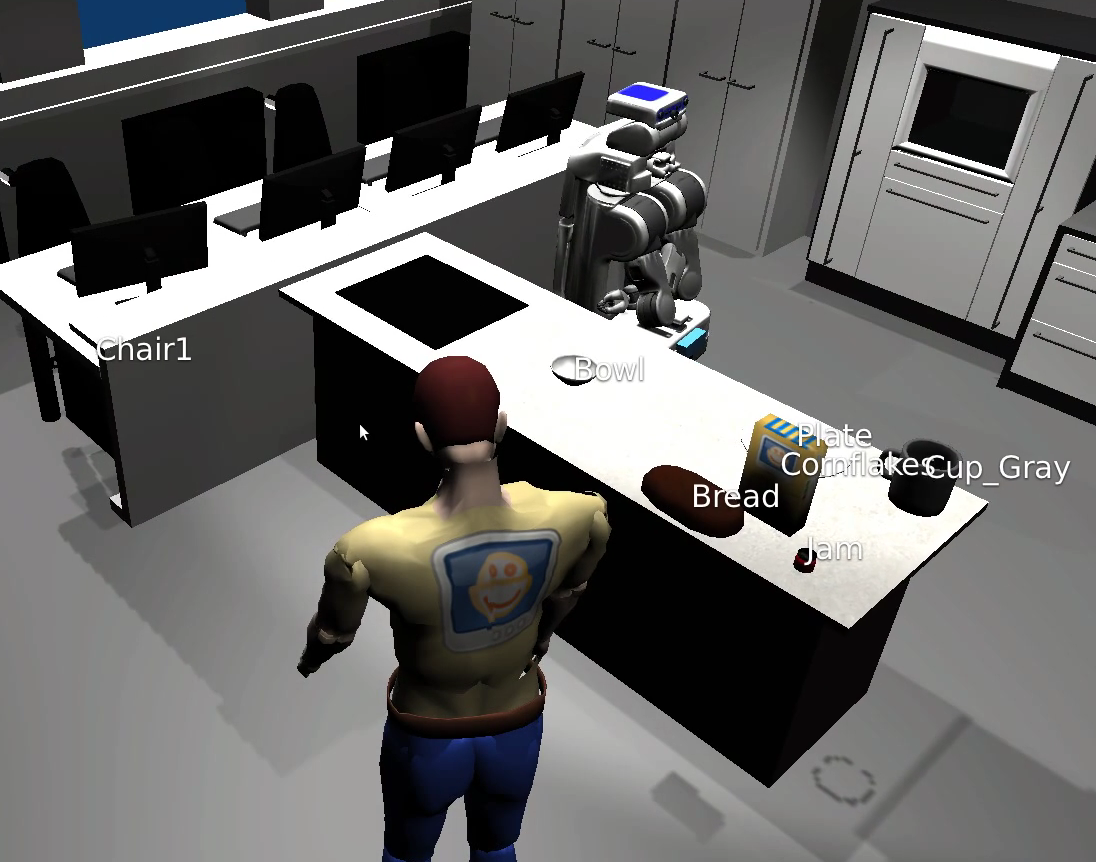
\includegraphics[width=0.475\textwidth]{pics/human_control_1.png} & 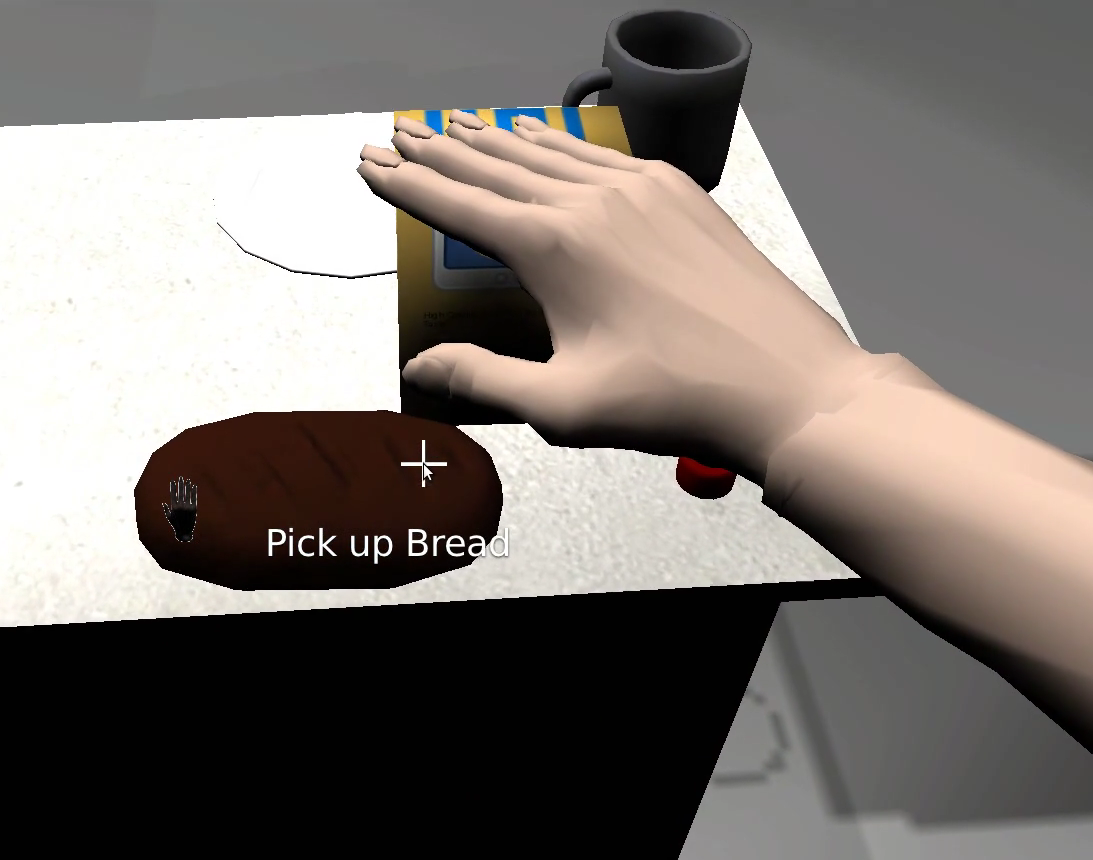
\includegraphics[width=0.475\textwidth]{pics/human_control_2.png}
\end{tabular}
\caption{The left picture shows a third-person view of the human component that is used to navigate in the environment. Here
objects, that the human can interact with, are displayed. The right picture shows the first-person perspective of the human 
avatar that indicates a possible ``pick-up-action'' with the bread.}
\label{fig:human_control}
\end{figure}

This computer-game like control enables users to perform pick- and place actions in simulated worlds using the 
human component of MORSE. At the same time, the robot(s) in the simulation can be controlled one of the robotic middlewares. 

The avatar can be controlled much like a character in a videogame, using either the mouse and
keyboard or a combination of the Microsoft Kinect and the Nintendo Wiimote. The
avatar can navigate around the environment, sit down on chairs and take objects
specifically marked as ``graspable''.



\section{Use Cases}
\label{section:usecases}

MORSE is currently being applied to test robotics algorithms mainly in two
different fields:

\textbf{Field robotics}: These experiments regard the deployment of more than
one robot in large outdoors environments. The terrain should not be initially
known to the robots, so they are expected to explore and navigate autonomously
as they carry out their mission.
The robots do not directly affect the environment, but have a large number of
sensors that allow them to navigate and accomplish specific objectives.

The Action \cite{6106782} project consists on the cooperation between ground
and air robots to locate and follow moving targets. The tests are done in
specific environments, which require transporting the robots a considerable
distance, always being dependant on the prevailing weather.  The use of
simulation offers the advantage of running the experiments regardless of the
weather, and not having to plan long trips to the actual experimental site.
Simulation also simplifies the execution of test runs, since they can be
restarted from the initial point within seconds.  Future stages of the project
require the coordination of larger teams of heterogeneous robots. The physical
robots required for these stages are not currently available, but simulation
permits for testing of these scenarios in advance.

Another project for outdoors robotics is Rosace
\cite{springerlink:10.1007/978-3-642-12384-9_18,springerlink:10.1007/978-3-642-28786-2_32}.
Its main objective is the coordination of robotic agents in search and rescue
operations in the case of a disaster. In this scenario, terrestrial robots must
be able to locate human victims, provide support for the victims and avoid
dangerous areas. The robots in the team are to be equipped with different
capabilities, and take autonomous decisions on which of them should perform
different tasks in the mission, such as searching, providing a communications
relay, and helping victims directly.  In the simulation, a source of fire, or
other dangers, can be added to the scenario, to train the robots on taking
preventive measures to avoid problems and protect the victims.
There are few robots available to do real experiments for this project. The use
of MORSE permits deploying large number of robots, with different payloads.
MORSE also permits giving some basic behaviour to the simulated human victims,
by scripting movement patterns and allowing them to visually show their
injured or healthy status by using different colors.


\textbf{Indoor service robotics}: In this scenario, complex robots are expected
to collaborate with humans to carry out ordinary household tasks, such as
cleaning, serving food or aiding humans to navigate an environment.
Robots used in these experiments are equipped with one or two arms, and are
capable of grasping objects. They are also expected to react to the actions of
their human collaborator, using video cameras, motion detectors or telemetry to
determine the location, pose and attitude of the human.

In MORSE, the robotic arms can be operated either by control of the end
effector and using Inverse Kinematics, or by direct control of the angles at
each joint.  The physics simulation using Bullet allows the detection of object
collisions.

To represent the human collaborator, a simulated avatar has been developed in
MORSE. By using game console controllers (Kinect and Wiimote), the user can
interact with the simulated environment. The simulated robot can then acquire
data about the pose of the avatar. This can be done at two different levels of
abstraction. Using the video cameras to recognise the human and its pose can be
done realistically, with the associated computational cost and uncertainties.
Alternatively, the avatar can directly export the position of all of its
joints, and feed them back to the robot, simulating a full motion capture
system and avoiding the processing costs.



%%%%%%%%%%%%%%%%%%%%%%%%%%%%%%%%%%%%%%%%%%%%%%%%%%%%%%%%%%%%%%%%%%%%%%
\section{Summary}
\label{section:discussion}


MORSE is developed as an open--source project, the source code can be
downloaded from the GIT repository:
(\url{http://github.com/laas/morse.git})

User documentation and additional information is also available at
(\url{http://morse.openrobots.org})


\subsubsection*{Acknowledgments}
This work has been partially supported by the DGA founded Action project
(\url{http://action.onera.fr}) and the STAE foundation Rosace project\\
(\url{http://www.fondation-stae.net})

% ---- Bibliography ----
\bibliographystyle{unsrt}
\bibliography{./morseBiblio}
\end{document}
